\setlength\parindent{0pt} % no indentation for the entire note
\subsection{total mass of a uniform parcel}
\begin{equation}
   M = n \big[\text{mole}\big] N_a \big[\frac{\text{molecule}}{\text{mole}}\big] m
       \big[\frac{\text{kg}}{\text{molecule}}\big]
\end{equation}
where the Avogadro's constant, $N_a = 6.022\times10^{23}$, is found by taking 12 grams of
$C^{12}$ and divide by the weight of a single $C^{12}$. It can also be found by taking 1 gram of 
$H^{1}$ and divide by the weight of a single $H^{1}$. We can thus define the molar mass for
$C^{12}$, $\mu = 12 \big[\frac{\text{g}}{\text{mole}}\big] = N_a m$, and the molecular mass of
$C^{12}, m = \frac{\mu}{N_a}$ [kg]. 

\subsection{temperature}
\begin{defn*} Temperature is heat generated by the mean kinetic energy (MKE) of molecules
\begin{equation}
   \frac{2}{3} k_B T = <\frac{1}{2} m u^2> + <\frac{1}{2} m v^2> + <\frac{1}{2} m w^2>,
\end{equation}
divide by the Boltzmann constant $k_B = 1.381 \times 10^{-23} J K^{-1}$. The one-to-one relationship
between temperature and MKE implies that the average (time average over a single molecule, or over
an ensemble of molecules) KE is always the same under the same macroscopic state. 
\end{defn*}

\subsection{pressure}
\begin{defn*} The statistical force of molecules over an area divide by the area. \\
\end{defn*}

\begin{derv*} 
Given the number density $\tilde{n} = \frac{n N_a}{V}$ (number of molecules per
unit volume) of a gas with x-velocity $u$. All molecules have varying velocity, hence we define the
number density $\tilde{n}_u$ indexed by a specific velocity $u$. The relationship between
$\tilde{n}$ and $\tilde{n}_u$ is
\begin{equation}
\begin{aligned}
   \tilde{n} & = \frac{n N_a}{V} \\
             & = \frac{\sum_{i}^\infty n_{u_i} N_a}{V} \\
             & = \frac{\int n_{u} du N_a}{V} \\
             & = \int \tilde{n}_u du.
\end{aligned}
\end{equation}
The force exerted by molecules with velocity $u$ at the x-direction walls recieving only $u$ is
\begin{equation}
   F_u = \tilde{n}_u u\delta t A \frac{2m u}{\delta t} = 2m\tilde{n}_u u^2 A.
\end{equation}
Integrating over all velocities and divide by the area, the pressure on the wall becomes
\begin{equation}
   p = \int 2m\tilde{n}_u u^2du = 2 \tilde{n} <m u^2>.
\end{equation}
Since this is the pressure exerted in x-direction on both wall added, so for a single wall we divide
by 2 and become 
\begin{equation}
   p = \tilde{n} <m u^2>.
\end{equation}
From the temperature definition we know that $<m u^2>=k_BT$, hence
\begin{equation}
   p = \frac{N}{V}k_B T.
\end{equation}
\end{derv*}

\subsection{ideal gas (equation of state)}
\begin{defn*} The ideal gas law 
\begin{equation}
   p V = n (N_a k_B) T = n R^* T
\end{equation}
where $R^* = 8.314$ J mol$^{-1}$K$^{-1}$. Dividing both sides by the mass $M = n N_a m$,
\begin{equation}
   \frac{p}{\rho} = \frac{R^*}{N_a m} T = R T,
\end{equation}
gives the specific gas constant $R$ ($R^*$ per unit molar mass). Set $M=M_d$, $m=m_d$, $p=p_d$ for the dry air, then 
\begin{equation}
   p_d = \rho_d R_d T,
\end{equation}
where $R_d = 287$ J kg$^{-1}$ K$^{-1}$. This also applies to water vapor
\begin{equation}
   e = \rho_v R_v T.
\end{equation}

\begin{figure}[H]
   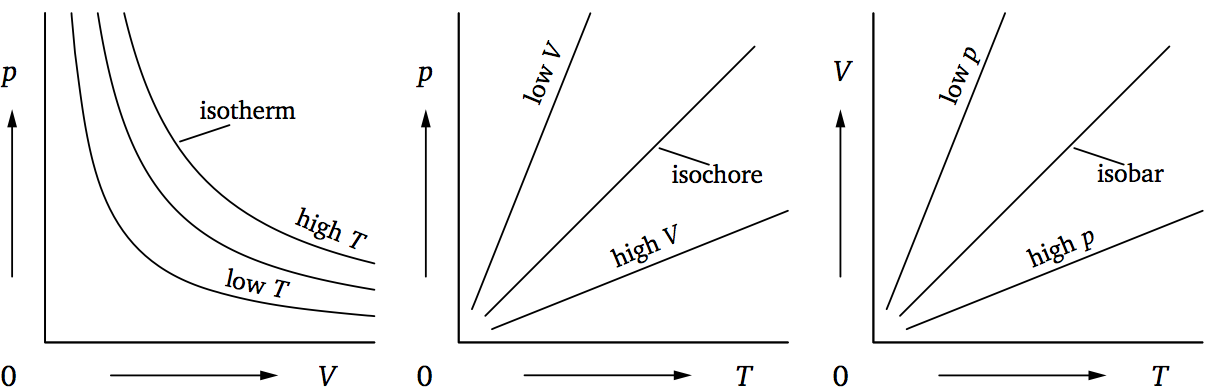
\includegraphics[width=1\textwidth, height=0.3\textwidth]{pVT.png}
   \caption{\label{fig:pVT}
      left to right: Boyle's Law, Gay-Lussac's Law and Charles's Law.}
\end{figure}
\end{defn*}



\subsection{state function}
\begin{defn*} $f(p,V,T)=0$.  A function that describes the \emph{equilibrium} state of a system (e.g., energy,
internal energy, enthalpy, entropy, pressure, temperature, volume, chemical composition, density,
etc) irrespective of how the system arrived in the state. 
\end{defn*}

\subsection{process function}
\begin{defn*} Values that depend on the \emph{path} (e.g., time) of two equilibrium states (e.g.,
work, and heat).
\end{defn*}



\subsection{internal energy}
\begin{defn*} $I(S,V,\{N_i\})$, composed of kinetic and potential energy of the molecules and
atoms, where chemical potential transfers to kinetic and temperature is proportional to kinetic
energy. The change depends only on the initial and final states of the system. Can not be directly
measured, but can be prepared by taking partial derivative of entropy, volume, and its mole number. \\
\end{defn*}

During a isothermal process with no change in volume (no work involved), then the
change in internal energy must be from heat exchange. If the system is adiabatic (no heat involved),
then the internal energy change must be from expansion/compression.

\subsection{internal energy (dry ideal gas)}
\begin{defn*} d$I = c_v$ d$T$, the internal energy soley depends on temperature, not
volume/density/pressure. \\
\end{defn*}


{Joule's experiment:} \\
In a free expansion ($p_iV_i = p_fV_f$, pressure change is completely balanced by volume change),
d$W = 0$, d$Q = 0$ hence d$I = 0$, and from the ideal gas equation the temperature stays constant
(since the molecules rarely meet even before the expansion, so the kinetic energy, which is affected
solely by temperature for ideal gas, remains constant). We can therefore conclude that internal
energy is solely governed by temperature. We can imagine this conclusion by using two Joule's
experiment by using the same volume compartment begining with two different temperatures, which
gives two internal energies in the end of expansion. 


\subsection{heat}
\begin{defn*} Heat is energy ``transferred" between two objects or systems in thermal contact, not
a state to a single system. Do not confuse heating rate as a time derivative of a function of state.
\end{defn*}


\subsection{heat (dry ideal gas)}
\begin{derv*} 
From first law of thermodynamics for a unit mass of dry ideal gas
\begin{equation} \label{eq:energy_cv}
\begin{aligned}
  \td Q & = \td I + \td W \\
        & = c_v \td T + p \td \alpha \\
        & = c_v \td T + \td(p\alpha) - \alpha \td p \\
        & = \td (c_v T + p\alpha) - \alpha \td p. 
\end{aligned}
\end{equation}
Original equation states that the heat change is due to internal energy change and work done by the
sytem/dry gas. The final equation first term is heat change due to change in {\bf{enthalpy}}, $h = I
+ p\alpha$, at constant pressure. Where change in internal energy/temperature and volume take
effect. The second term is heat change at constant temperature due to pressure change (heat increase
causes initial molecular momentum to increase/pressure increase, but if temperature stays constant
the volume must expand ($pV=Nk_BT$), thus final pressure decreases). Further derivation 
\begin{equation} \label{eq:energy_cp}
\begin{aligned}
  \td Q & = (c_v + R) \td T - \alpha \td p
        & = c_p \td T - \alpha \td p
\end{aligned}
\end{equation}
shows that the heat capacity under constant pressure and constant volume could be associated by
\begin{equation}
  \big( \frac{\td q}{\td T} \big)_p = \frac{\td h}{\td T} =  c_p = c_v + R.
\end{equation}
\end{derv*}

\subsection{potential temperature (dry ideal gas)}
\begin{defn*} $\theta = \big(\frac{p_0}{p}\big)^\kappa$, this is obtained by setting $\td Q=0$
and integrate \eqref{eq:energy_cp}. 
\end{defn*}

\subsection{(saturation) equivalent potential temperature}
\begin{defn*} $\theta_e$, the temperature obtained by condensing out all the vapor. \\
\end{defn*}

\begin{derv*} 
From first law, 
\begin{equation}
\begin{aligned}
   \td Q & = c_p \td T - \alpha \td p \\ 
         & = c_p \td T - RT \td \ln p \\
         & = c_p( \td T - \frac{RT}{c_p} \td \ln p) \\
         & = c_p( \td T + T \td \ln(\frac{p_0}{p})^\kappa) 
\end{aligned}
\end{equation}
when substituting $\td Q = -L\td q_{s}$ (the negative means evaporative cooling of the parcel when
$q_{s}$ increases, otherwise condensative heating) and divide by $c_p T$ this becomes, 
\begin{equation} \label{eq:saturationCooling}
\begin{aligned}
   \frac{-L}{c_pT} \td q_{s} & = \td \ln T + \td \ln(\frac{p_0}{p})^\kappa \\
          & = \ln (T(\frac{p_0}{p})^\kappa) = \td \ln \theta.
\end{aligned}
\end{equation}
Integrate from saturation to all moisture condensed out ($q_{s}=0$) results in the equivalent potential
temperature
\begin{equation}
\begin{aligned}
   \boxed{\theta_e = \theta\exp(\int_0^{q_{s}} \frac{L}{c_pT} \td q_{s}) 
         \approx \theta\exp(\frac{L}{c_pT} q_{s})}.
\end{aligned}
\end{equation}
Where the approximation is due to saturated vapor mixing ratio decreasing much faster than
temperature with height (see Wallace and Hobbs p107). 
\end{derv*}

\subsection{liquid water potential temperature}
\begin{derv*} 
Replace the lhs of \eqref{eq:saturationCooling} with liquid water which just
reverses the process/sign 
\begin{equation}
\begin{aligned}
   \boxed{\theta_L \approx \theta\exp(-\frac{L}{c_pT} q_{L})}.
\end{aligned}
\end{equation}
This can be further approximated by the first-order/linear power series of
exponential (\cite{betts1973non}, \cite{grenier2001moist})
\begin{equation}
   \boxed{\theta_L = \theta(1 - \frac{L}{c_pT} q_{L})}.
\end{equation}
\end{derv*}


\subsection{continuity of water}
\begin{derv*} 
The water vapor for example has
\begin{equation}
\begin{aligned}
   \frac{D q_v}{D t} & = \frac{D}{D t} (\frac{\rho_v}{\rho_d}) \\
        & = \frac{-\rho_v}{\rho_d^2} \frac{D \rho_d}{D t} + \frac{1}{\rho_d}\frac{D \rho_v}{D t} \\
        & = \frac{\rho_v}{\rho_d^2}(\rho_d \nabla \cdot v) - \frac{1}{\rho_d}(\rho_v \nabla \cdot v) \\
        & = 0,
\end{aligned}
\end{equation}
where the second equality uses mass continuity ($\frac{D \rho}{D t} = -\rho \nabla\cdot v$). Thus,
with sources and sinks ($\dot{S}$) becomes
\begin{equation}
   \frac{D q_v}{D t} = \dot{S}.
\end{equation}
The $n$ species of water can be expressed as
\begin{equation}\label{eq:cont_w}
   \boxed{\frac{D q_i}{D t} = \dot{S_i}, \ i=1,\dotsc,n}.
\end{equation}
\end{derv*}



\subsection{thermodynamic equation}
For general {\clr non-ideal gas}, by combining continuity equation and
\begin{equation}
    \frac{DI}{Dt} + p \frac{D\alpha}{Dt} = \dot{Q}, 
\end{equation}
results in the internal energy equation
\begin{equation}
    \boxed{\frac{DI}{Dt} + p\alpha \nabla \cdot v = \dot{Q}}.
\end{equation}
and the pressure term (also missing the dynamics in the momentum equation) could be obtained
diagnostically as
\begin{equation} 
   p = -\frac{\partial I}{\partial \alpha},
\end{equation}
where $\alpha$ dynamics is from continuity equation. \\

As for {\clr ideal gas}, 
\begin{equation}
    c_v\frac{DT}{Dt} + p \frac{D\alpha}{Dt} = \dot{Q}, \ \text{or} \ \ 
    c_p\frac{DT}{Dt} + \alpha \frac{Dp}{Dt} = \dot{Q},
\end{equation}
one would obtain a thermodynamic equation for $T$ and solve for $p$ by $p = \rho R T$. Which is
by combining the continuity equation with
\begin{equation}
    \frac{DI}{Dt} - \frac{RT}{\rho} \frac{D\rho}{Dt} = \dot{Q},
\end{equation}
and result in the temperature equation
\begin{equation}
    \boxed{c_v\frac{DT}{Dt} + RT \nabla \cdot v = \dot{Q}}.
\end{equation}
If further large scale \emph{\clr hydrostatic balance} $\alpha \td p = -g \td z$ is assumed, then
the thermodynamic equation pertains to the dry static energy $\td Q = \td (c_v T + gz) = \td s$, 
\begin{equation}
   \boxed{\frac{Ds}{Dt} = \dot{Q}}.
\end{equation}
According to \eqref{eq:cont_w}, if the rhs tendency comes from water vapor (see
\cite{khairoutdinov2003cloud} for more details)
\begin{equation}
   \boxed{\frac{Ds}{Dt} = -L_v\frac{Dq_v}{Dt}}
\end{equation}
then there must be sources/sinks of vapor evaporative cooling/condensative heating.
The negative sign is explained by supposing there is positive (negative) $dq_v$, which is increasing
(decreasing) the vapor in the parcel, this means that the there must be evaporative cooling
(condensative heating) to the parcel.


\subsection{reversible process}
In thermodynamics term, a process ``taken place" is defined as transition from intial to final
state. A reversible process is if this process can be reversed without additional work, and causes
no change to the system or surrounding environment. 

\subsection{entropy}
A measure of ``difference'' between adiabats (no heat exchange processes), and a measure of ``work
loss'' in transferring heat (irreversible process). \\

In a closed system, when heat is added at a constant temperature (volume expands and pressure
decreases), the amount of disorder increases which increases the potential temperature (the actual
temperature is higher when forced back to original pressure). For a irreversible process, suppose a
heat reservoir at $T_2$ transfers heat $Q$ to a cooler reservoir at $T_0$. By Carnot's engine, we
know that the maximum available energy the heat tranferred into work is
\begin{equation}
    W_2 = (1-\frac{T_0}{T_2})Q.
\end{equation}

For a irreversible process (state variables (e.g., p, V, T) cannot go back to original values
without additional work), where heat is first transferred to a middle reservoir at the state $T_1 <
T_2$, and then transfers the same amount of heat $Q$ to the cold reservoir at $T_0$.
Notice since $T_1 < T_2$, therefore the entropy is higher to transfer the same amount of $Q$.
Therefore the maximum available work from the middle reservoir is
\begin{equation}
    W_1 = (1-\frac{T_0}{T_1})Q,
\end{equation}
which is less than $W_2$. Hence, the work loss from irreversible process is 
\begin{equation}
    W_2-W_1 = Q(T_0/T_1 - T_0/T_2) = T_0(S_1 - S_2) = T_0 dS,
\end{equation} 
in a form of heat loss, where the increase in $dS$ becomes a measure of work loss. 
%A sum of entropy gain of $S_1$ from the middle reservoir and 
%entropy loss of $S_2$ from the original reservoir in the irreversible process.
There is a net gain in entropy in the irreversible process.
i.e., {\bf the more entropy gain/more disorderness contributes to more work loss, which becomes a
less efficient process.}

\subsection{specific volume}
\begin{defn*} $v = 1/\rho$, volume occupied by 1kg of mass.
\end{defn*}

\subsection{mixing ratio}
\begin{defn*} $ \frac{m_i}{m_{\text{tot}}-m_i} $.
\end{defn*}

\subsection{vapor mixing ratio}
\begin{defn*} $ q = \frac{m_v}{m_d}$, actual mass mixing ratio between vapor and dry air.
\end{defn*}

\subsection{saturation mixing ratio}
\begin{defn*} $ q_s = \frac{m_{vs}}{m_d}$, maximum amount of water vapor allowed in the dry air.
\end{defn*}
\begin{derv*} 
\begin{equation}
\begin{aligned}
   q_s & = \frac{m_{vs}}{m_d} \\
       & = \frac{e_s/(R_v T)}{(p-e_s)/(R_dT)} \\
       & = 0.622\frac{e_s}{p-e_s} \\
       & \approx 0.622\frac{e_s}{p}
\end{aligned}
\end{equation}
where $p >> e_s$ in the atmosphere.
\end{derv*} 

\subsection{latent heat}
\begin{defn*} $Q$ [kJ], energy released/absorbed by a body during a constant temperature process
(phase transition).
\end{defn*}

\subsection{specific latent heat}
\begin{defn*} $L$ [kJ/kg]= $Q/M$, amount of heat required to complete phase change of a unit
mass of substance.
\end{defn*}

\subsection{Clausius-Claperon Relation}
\begin{defn*} $\frac{\Delta P}{\Delta T} = \frac{L}{T\Delta v}$, P-T coexistence curve slope
relation. Under typical atmoshperic conditions, 
\begin{equation}
   \frac{d e_s}{dT} = \frac{L_v(T)e_s}{R_vT^2}, 
\end{equation}
where: $L_v$ is latent heat for evaporation varying with $T$, $R_v$ is the water vapor gas constant.
\end{defn*}


\subsection{saturation vapor pressure}
August-Roche-Magnus formula (approximation from Clausius-Claperon Relation): \\
\begin{equation}
   e_s(T) = 6.1094 \text{exp}(\frac{17.625T}{T+243.04}).
\end{equation}
( water-holding capacity of the atmosphere increases by about $7\%$ for every $1^{\circ}$C heated )

\subsection{unsaturated vapor pressure}
\begin{defn*} $e = \frac{(n_{\text{air}} + n_{\text{water}})}{V}RT$, 
\end{defn*}

\subsection{relative humidity}
\begin{defn*} $RH = \frac{e}{e_s}(T)$.
\end{defn*}

\subsection{virtual temperature}
\begin{defn*} 
$T_v(p,\rho)$, temperature at which a dry parcel would have at $p$ and $\rho$ of a moist parcel. 
\end{defn*}

\begin{derv*} Suppose a moist parcel has density $\rho$ and pressure $p$.
Dalton's law of partial pressure gives $p = e + p_d$, combined with \eqref{eq:idealgas2} and
\eqref{eq:idealgas3} give
\begin{equation}
   \rho = \frac{M_d + M_v}{V} = \rho_d + \rho_v = \frac{p-e}{R_dT} + \frac{e}{R_vT}, 
\end{equation}
where $\rho_d$ and $\rho_v$ are the partial densities.
Solving this gives
\begin{equation}
   {\clr p} = {\clr \rho} R_d \frac{T}{1-\frac{e}{p}(1-\frac{R_d}{R_v})} = \rho R_d {\clr T_v},
\end{equation}
where, $\frac{R_d}{R_v} \approx 0.622$ in the atmosphere. \\
\end{derv*}
This can be written as a function of specific humidity
\begin{equation}
   T_v = T(1 + 0.61q). 
\end{equation}
The gas constant for moist air (a mix of pure water vapor and dry air) depends strongly on the
amount of water vapor, so it is convenient to use a fictitious temperature with the dry-air equation
of state to represent how "heavy" a moist parcel is (i.e., the more water vapor means a dry air
needs to heat more to reach same pressure and density to become "light"). \\


\subsection{virtual potential temperature}
\begin{defn*}
$\theta_v = T_v (\frac{p_0}{p})^\kappa$, and $\theta_v = \theta(1+0.61q)$, by using dry air
constant, the virtual potential temperature is just the potential temperature using $T=T_v$, 
\end{defn*}




\subsection{lifting condensation level (LCL)}
\begin{defn*} $z_l$, height at which an unsaturated parcel reaches saturation, $RH=100\%$, dry
adiabatically, then starts following moist adiabatic lapse rate upward. 
\begin{figure} [H] 
   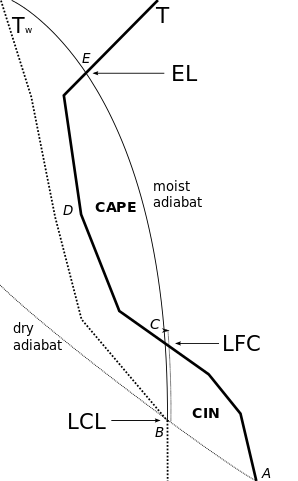
\includegraphics[width=0.2\textwidth, height=0.3\textwidth]{sounding.png}
   \caption{\label{sounding}}
\end{figure}
\end{defn*}

\subsection{level of free convection (LFC)}
\begin{defn*} $z_f$, height at which a moist parcel temperature is equal to the environment,
and temperature increases faster than the environment. 
\end{defn*}

\begin{exmp*} 
The unsaturated parcel in Figure {\ref{sounding}} is lifted dry adiabatically from A
to B to saturation, and further lifted moist adiabatically to C until surpassing the environmental
temperature.
\end{exmp*}

\subsection{equilibrium level (EL)}
\begin{defn*} $z_e$, height at which the moist parcel lapse rate is greater than environment.
\end{defn*}

\subsection{dew point/condensate temperature}
\begin{defn*} $T_d$, temperature at LCL when a parcel reaches $RH=100\%$ by expansion cooling.
\end{defn*}

\subsection{wet bulb temperature}
\begin{defn*} $T_w$, the temperature when saturation is reached in a bulb of moist ambient air
and a wet cloth through evaporative cooling, i.e., air cooled by cloth warming (measure taken from
the air). 
\end{defn*}

$T_w$ is reached by evaporative cooling, whereas $T_d$ is reached by expansion cooling (constant
pressure). $T_d \le T_w$ since when a parcel saturates by evaporation, the dew point inside
increases which is higher than the original dew point $T_d$.

\subsection{convective inhibition (CIN)}
\begin{defn*} 
CIN $=\int_{z_0}^{z_f} g \frac{T_{v,\text{parcel}} - T_{v,\text{env}}}{T_{v,\text{env}}} $d$z$, 
a negative energy value measuring how much a parcel is prevented to rise to LFC from the surface. \\
\end{defn*}

The term $\frac{T_{v,\text{parcel}}}{T_{v,\text{env}}} - 1$ shows when the parcel is moister (larger
$T_{v,\text{parcel}}$, more buoyant), CIN is less negative.

\subsection{convective available potential energy (CAPE)}
\begin{defn*} 
CAPE $=\int_{z_f}^{z_e} g \frac{T_{v,\text{parcel}} - T_{v,\text{env}}}{T_{v,\text{env}}} $d$z$,
differs from CIN in just the levels of integration.
\end{defn*}


\subsection{Reynolds number}
\begin{defn*}
%
\begin{equation}
   \text{Re} = \frac{\text{inertial forces per unit area}}{\text{viscous forces per unit area}} =
   \frac{\rho v L}{\mu} = \frac{v L}{\nu} 
\end{equation}
%
where $v$ is the maximum speed of the object relative to the fluid.
\end{defn*}
